\documentclass[twocolumn]{article}
\usepackage[fleqn]{mathtools}%for aligning parameters of fitted erfc(x)
\usepackage{geometry}	%
\usepackage{abstract} %to get email footnotes
\geometry{margin=2cm}	%more visible figures (more place) 
\usepackage[superscript,biblabel]{cite}%superscript citing
\usepackage[utf8]{inputenc}
\usepackage[english]{babel}
\usepackage{amsmath}	%booklet
\usepackage{hyperref}	%clickable citings, referencing URL via \url{}
\usepackage{siunitx}	%for SI units; see ftp://ftp.dante.de/tex-archive/macros/latex/exptl/siunitx/siunitx.pdf
\usepackage{graphicx} 	%includegraphics
\usepackage{mhchem}		%writing chemical elements with mass numbers
\usepackage[nottoc]{tocbibind}	%references
\usepackage{indentfirst}%indenting first paragraphs

%the command \insertFigure{file} inserts figure with width 0.9*(column width)
\newcommand{\insertFigure}[1]{%
   \includegraphics[width=0.95\linewidth]{#1}%
}

\title{\textbf{A248: Magneto-optical Trap}}
\author{Bence Mitlasóczki\thanks{s6bemitl@uni-bonn.de} and Beno\^it Scholtes\thanks{s6bescho@uni-bonn.de} \\ \textit{Rheinische-Friedrich-Wilhelms Universit\"at Bonn}}
\begin{document}
\renewcommand{\abstractname}{\vspace{-\baselineskip}} %supresses abstract title
\twocolumn[ %makes a one column abstract
\begin{@twocolumnfalse}
\maketitle

\begin{abstract} \vspace{-8mm}
We adjusted some mirrors to get MOT. We did some measurements.
\end{abstract}
\end{@twocolumnfalse}
\hspace{5mm} ]
\maketitle
\saythanks %from abstract package to ensure email footnotes from \thanks command in a two-column article
\section{Introduction}
Magneto-optical traps (MOT) are an important apparatus in modern atomic physics experiments, used to slow and trap a neutral atom cloud to temperatures as cold as several microkelvin. They are achieved by combining radiation pressure from laser beams and a quadropole magnetic field inside a vacuum cell rid of other gasses. Their use ranges from probing atomic properties, quantum optics, cold collision, quantum information processing, and acting as the preliminary stage to achieving even colder atom traps, namely Bose-Einstein condensates. This experiment aimed at obtaining a MOT and finding its size, population, and loading behaviour as well its fluorescence dependence on the magnetic field strength, quarter waveplate angle, and laser frequency detuning.

\section{Theory}
The central process by which atomic gasses are cooled are via radiation pressure from lasers. When a photon is absorbed by an object, particle, or atom, its energy as well as its momentum, equal to $p=\hbar k$, is absorbed as a result of momentum conservation. This radiation pressure can be used to slow down moving atoms if the atoms absorb photons travelling in the opposite direction. The atoms are thus cooled due to the decrease in their kinetic energy, which is proportional to their temperature. Only photons resonant to a transition of the absorption spectrum of the atoms are absorbed however. As a result, the absorption spectrum of the atoms to be cooled needs to be known and a particular transition chosen such that the required frequency of the cooling laser can be determined. The absorption spectrum of $^{85}\ce{Rb}$ and the transition used is discussed in Section~\ref{sec:Rubidium}. \\

\par A moving atom will no longer be able to absorb photons with frequencies from the absorption spectrum however, as their frequency will be Doppler shifted and no longer resonant to the atom transitions. The moving atom will only be able to absorb light which has been Doppler shifted such that it is resonant with one of its excitation transitions. In an uncooled gas, the atoms are all travelling in different directions with different speeds. As a result, light incident on the gas from a single direction will be Doppler shifted differently for all the different atoms. An absorption spectrum obtained from such a gas will thus be Doppler broadened, making it difficult to determine the energy levels and transitions of the atoms. In order to obtain a spectrum with high resolution, Doppler-free spectroscopy such as saturation spectroscopy needs to be used. 

%In order to obtain a MOT, two lasers are used. A cooling laser is used to actively slow and thus cool the atoms down, while a repumping laser is used to `repump' rare atoms that have excited to off-resonant states back into states that can be slowed by the cooling laser. The repumping laser will be explained in Section~\ref{sec:Rubidium}. Figure~\ref{fig:Laser} shows the setup for the preperation of the two lasers for the MOT.
%TODO talk about Doppler and natural broadening of spectrum, Voigt-profile
\subsection{Saturation Spectroscopy}
Atoms can only absorb photons with frequencies that are resonant to their excitation transitions. That said, a moving atom will not be able to absorb photons with these frequencies as their frequency will be Doppler shifted and no longer resonant to the atom transitions. The moving atom will only be able to absorb light which has been Doppler shifted such that it is resonant with one of its excitation transitions. In an uncooled gas, the atoms are all travelling in different directions with different speeds. As a result, light incident on the gas from one direction will be Doppler shifted differently for all the different atoms. An absorption spectrum obtained from such a gas will thus be Doppler broadened, making it difficult to determine the energy levels and transitions of the atoms. In order to obtain a spectrum with high resolution, Doppler-free spectroscopy such as saturation spectroscopy needs to be used. \\
Saturation spectroscopy utilises two lasers, called the pump and test beams, which are incident on the gas in opposite directions. The test beam is much less powerful and its intensity after passing through the gas is measured~\cite{manual}. The absorption spectrum measured in this manner will largely look like a Doppler broadened spectrum, though with sharp peaks in the middle of Doppler broadened peaks as seen in Figure~\ref{fig:Lamb}. These are a result of the intense pump beam directed in the opposite direction though always with the same frequency as the test beam. Only atoms stationary along the axis of the lasers will be resonant to both the pump and test beam for a given transition as the Doppler shifts of either laser is always different for moving atoms. As a result, when the pump and test beam are resonant to an excitation transition, the pump beam will saturate the stationary atoms by exciting most of them to higher states, leaving few left for the test beam to excite. Thus the test beam will be measured with a much less diminished intensity than was measured for other frequencies, where the atoms saturated by the pump beam were not those resonant to the test beam. Thus a peak in the Doppler broadened absorption spectrum is observed, called a Lamb dip. These peaks provide the Doppler-free absorption spectrum of the gas. A crossover peak is observed when the pump and test beam are both resonant to atoms moving at such a velocity that two different hyperfine transitions are individually resonant to both beams. Here, the pump beam excites many atoms to a certain state, thereby depopulating the ground state of these atom and again leaving few left for the test beam to excite. This leads to more peaks in the absorption spectrum than the number of transitions.
\begin{figure} [!h]
	\centering
	\insertFigure{Images/Lamb.png}
	\caption{A Lamb dip observed in a Doppler-broadened absorption peak.~\cite{manual}}
	\label{fig:Lamb}
\end{figure}
\iffalse%written by Bence
\par Saturation spectroscopy makes use of two beams, often from the same source: the powerful pump beam and a weaker probe beam, passing through the sample in opposite directions. Due to the Doppler-broadened spectrum of the ensemble, there will be absorption in the wider frequency region for each beam, corresponding to a group of atoms (velocity class) which move with the right velocity in the beam direction.  As the frequency of the two beams matches, while their direction is opposite, the corresponding velocity classes move with velocities $\pm v$ along the common beam axis. If $v = 0$, that is, the laser frequency matches the transition frequency without doppler-shift, the probe beam shows a drop in the absorption signal (difference of original probe beam intensity and detected transmitted intensity), which is called the Lamb dip (a peak in the transmission spectrum). The narrowness of the Lamb dip compared to the Doppler-broadening allows for a much higher resolution.
An important phenomenon is the appearance of crossover peaks: these appear at the middle frequency of two close peaks with an intersection in their Doppler-broadened spectra. The two beams interact with the same velocity class, but producing the two different hyperfine transitions.
\fi

\subsection{Polarisation Spectroscopy}%Laser Spectroscopy p. 464 (485)
Polarization spectroscopy is based on saturation spectroscopy. The pump beam is circularly polarized by passing through a quarter waveplate before entering the sample. This can be shown to introduce anisotropy\cite{demtroder}$^{(\text{p.}\,465)}$ in the orientations of the angular momentum $J$ of the atoms, the sample becomes birefringent.
In the realised setup, the probe beam is split in two by a polarizing beam splitter (PBS),
only one of them passing through the anisotropic sample, turning its polarization axis slightly. After entering the detector, the difference of the signals is formed, which shows the axis shift. The result is a dispersive signal with a shape similar to what is shown on Figure \ref{fig:Dispersive}. The zero crossing with differing voltage signs on the two sides provides a precise locking point for the laser frequency.
\begin{figure}
\centering
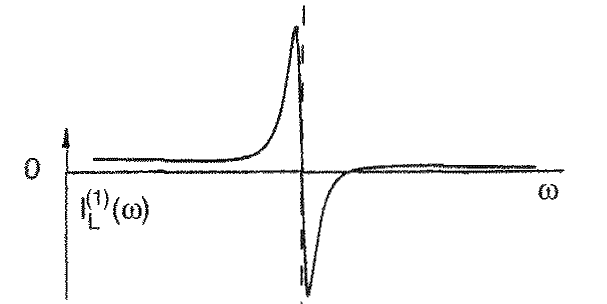
\includegraphics[scale=0.3]{Images/Dispersive.png}
\caption{A dispersive signal.\cite{demtroder}$^{(\text{p.}\,461)}$}
\label{fig:Dispersive}
\end{figure}

%TODO just talk about polarisation spectroscopy here and the resulting signal. Then mention that this is used here in order to use the signal for the error signal to lock the laser. Reference the section.

\subsection{Optical Trap}
An optical trap is organised with three lasers for the three directions of space, orientated so that they have a crossing point. Each laser is then reflected back into the gas and through this central crossing point so that there are six counter-propagating beams. This provides radiation pressure in six different directions, all directed back toward the crossing point. That said, the radiation pressure should only be imposed on atoms moving away from the trap. Otherwise, the lasers would also push out atoms in the trap and along the laser beam. As a result, the lasers are all red detuned from a particular transition such that when the atoms are moving away from the trap, these lasers are blueshifted for the atoms and become resonant with the transition allowing for the absorption of the photons. That said, the resonance of the atoms with the lasers is dependent on the velocity of the atoms. Furthermore, the probability of an atom absorbing a photon is dependent on the difference between the Doppler shifted frequency of the photon and the atom's transition frequency, as show in Figure~\ref{fig:Scat}. It can be seen that more atoms moving away from the centre will be forced back than atoms moving toward the centre. That said, using only one frequency for the lasers means that many atoms moving away from the centre of the trap will still be largely transparent to the lasers due to small scattering rates. The optical trap purely achieves an ``optical molasses" in the intersection volume of the lasers, so called because atoms moving away from the centre are slowed as if moving in a viscous medium. This molasses cannot completely stop the atoms from leaving the intersection volume however, whereby they will be lost to the trapping method, nor does it provide a point that the atoms are drawn towards. As a result, using the optical trap in conjunction with a magnetic trap is a better method.
\begin{figure} [!h]
	\centering
	\insertFigure{Images/Scat.png}
	\caption{The scattering rate and thus force from radiation pressure between the differently Doppler shifted laser photons and the atoms.~\cite{Wieman}}
	\label{fig:Scat}
\end{figure}
%TODO Do we need the equation of the force and excitation/scattering rate?

\subsection{Magneto-optical Trap}
A magnetic field is used to introduce a position-dependent force from radiation pressure. Two coils are arranged in an anti-Helmholtz configuration (face to face but with currents in opposing directions) to produce a quadrupole magnetic field, pictured in Figure~\ref{fig:mag}. 
\begin{figure} [!h]
	\centering
	\insertFigure{Images/Mag.png}
	\caption{A quadrupole magnetic field in 2D space. The field lines become more dense further from the centre, showing the increase in magnetic field strength.~\cite{mag}}
	\label{fig:mag}
\end{figure}
This magnetic field has a strength that increases linearly from centre, which itself has zero magnetic field. This means that the Zeeman effect, which splits previously degenerate magnetic energy levels of atoms into non-degenerate states with separation proportional to magnetic field strength $\Delta E \propto m_iB$ (where $m$ is the magnetic quantum number), increasingly separates energy levels the further from the centre an atom is. The lasers can thus be red detuned from one of these transitions such that as an atom moves away from centre, the transition becomes increasingly resonant with the laser, increasing the scattering rate. As a result, the force felt by atoms moving away from the centre of the intersection volume increases with distance, such that atoms can be more effectively trapped. This also ensures that atoms in centre of the volume will be largely transparent to the cooling lasers, as there is no magnetic field. Figure~\ref{fig:Zeeman} illustrates the Zeeman effect and resulting force on the atoms on either side of the trap. 
\begin{figure} [!h]
	\centering
	\insertFigure{Images/Zeeman.png}
	\caption{The Zeeman effect on atoms on either side of the centre where the magnetic field changes sign. The transitions allowed for differently polarised light is also shown.~\cite{Wieman}}
	\label{fig:Zeeman}
\end{figure}
As the magnetic field has a different sign on either side of the centre, a certain energy level $m_i$ will not have the same energy on either side. Circularly polarised lasers therefore need to be used, where the reflection of a laser will cause the polarisation to flip from $\sigma_-$ to $\sigma_+$ for example. The counter-propagating laser beams are thus oppositely polarised meaning that they will be resonant with different transitions, one with $m=-1$ and the other with $m=+1$. This is due to the transition selection rules where a $\sigma_\pm$ polarised photon requires that $\Delta m=\pm1$ between the initial and final states of the atom.~\cite{Foot} Though the beams are resonant to different transitions, these transitions will have the same energies the same distance away from the centre, meaning that a laser with a single frequency can become increasingly resonant atoms on either side of the atom trap. The magnetic field has thus introduced a point which the atoms are drawn towards. The complete MOT setup is given in Figure~\ref{fig:MOT2}. The centre of the magnetic field is to be aligned with the centre of the intersection volume of the lasers to achieve the best results. \\
\begin{figure} [!h]
	\centering
	\insertFigure{Images/MOT2.png}
	\caption{The MOT setup, shown with the coils in anti-Helmholtz configuration, magnetic field, and laser beam polarisations.~\cite{Foot}}
	\label{fig:MOT2}
\end{figure}
 
\par There is a limit to the extent that a MOT can cool down atoms. The atoms must always re-emit the energy that they have absorbed from the lasers. These photon emissions are isotropic however, leading to an average recoil force on the atom of $\langle F\rangle_{\text{recoil}}=0$~N, retaining the efficiency of the optical trap method. The atoms will nevertheless be pushed around randomly by the recoil forces during each photon emission, thus meaning that the kinetic energy and consequently temperature of the atoms will not be able to be further reduced past this point. This minimum temperature is called the Doppler limit, which is generally in the $\mu K$ for an MOT. Methods such as Bose-Einstein condensation must be used to cool down atom traps further. 

\subsection{Rubidium} \label{sec:Rubidium}
Natural Rubidium gas is composed of $^{85}\ce{Rb}$ and $^{87}\ce{Rb}$. This experiment focuses on $^{85}\ce{Rb}$ as it is approximately three times more abundant in the gas. The level structure of $^{85}\ce{Rb}$ is given in Figure~\ref{fig:Spectrum}. The transition used in this experiment for resonance with the cooling lasers with $\sigma_+$ polarisation is the F=3 (or m=3) $\to$ F'=4 transition. This transition is nominally closed meaning that excited atoms can only decay down into the F=3 state. This means that are continuously able to absorb photons from the cooling lasers, allowing for further cooling and trapping. There are rare excitations to the F'=2,3 states however which can decay to the F=2 ground state which is no longer resonant to the cooling lasers. As a result, a repumping laser tuned to the F=2 $\to$ F'=3 transition is introduced to pump atoms back into states sensitive to the cooling lasers when they decay to the F=3 state. One should note that $^{87}\ce{Rb}$ is still present in the gas and thus its spectrum will be visible.
\begin{figure} [!h]
	\centering
	\insertFigure{Images/Spectrum.png}
	\caption{The energy levels $^5S_{1/2}$ and $^5P_{1/2}$ of $^85\ce{Rb}$. The cooling laser and repumping laser transitions used are the F=3 $\to$ F'=4 and F=2 $\to$ F'=3 transitions respectively.~\cite{Wieman}}
	\label{fig:Spectrum}
\end{figure}

\section{Experimental setup} \label{sec:Exp}
\begin{figure} [!h]
	\centering
	\insertFigure{Images/Laser.png}
	\caption{The dependency of MOT luminosity on the current flow through the coils and thus the strength of the magnetic field.\cite{manual}}
	\label{fig:Laser}
\end{figure}
\subsection{Diode Laser}
The lasers used in the experiment are diode lasers. The reason for using this type of lasers is for two reasons: first, the state transitions we exploit (cooling and repumping) lie in the infrared range (Figure \ref{fig:Laser}), second, we need tunable coherent light sources.\\
Recombination of an electron with a hole in a diode may result in electromagnetic radiation, with a large linewidth.\cite{demtroder} In the laser diode, the metal case for heat dissipation and optical cavity makes it possible that above a threshold current, population inversion can occur, which means lasing with a large free spectral range (below the threshold, the diode acts as a LED). The resonator modes can be shifted by changing the temperature (externally or by changing the diode current): the band gap, the index of refraction and the length of the cavity change. We only changed the current throughout the experiment; the temperature change of the room influenced our setup, causing a slow drift. To use it in single mode, the laser is used in Littrow configuration, where an external grating is utilised. The grating is positioned such that for the desired frequency, the $-1.$ order is reflected back into the active medium, thus it serves as an external resonator element. The actual beam produced for use is the $0.$ order. For constructive interference, the grating equation reads\cite{demtroder}$^{(\text{p.}\, 114)}$ with the notation of Figure \ref{fig:Grating}:
\begin{equation}
2 d \sin \alpha = m \lambda\nonumber
\end{equation}
A piezo system functioning on triangular supply voltage is responsible for the moving of the grating, scanning through the laser spectrum.
\begin{figure}
	\centering
	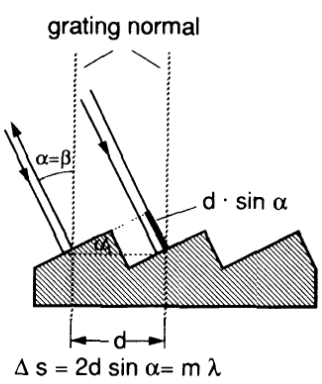
\includegraphics[scale=0.3]{Images/Grating.png}
	\caption{Diffraction grating in the special case when the incident and reflected beams coincide.\cite{demtroder}$^{(\text{p.}\, 114)}$}
	\label{fig:Grating}
\end{figure}
\begin{figure} [!h]
	\centering
	\insertFigure{Images/Diode.png}
	\caption{The diode laser with the grating in Littrow configuration.\cite{manual}}
	\label{fig:Diode}
\end{figure}
%Subsection Laser Detuning is not necessary in my opinion, being already explained in subsection Optical Trap
\subsection{MOT setup}
The actual realisation of the MOT system is presented herein short.\\
A vacuum chamber held at HV (high vacuum) pressure levels ($\approx 10^{-7}$~mbar) with glass windows and a Rb source inside served as the container for the vapor. The cooling and repumping beams were directed by an optical cable, two beam splitters, several mirrors and a quarter wave plate for each six directions of illumination. The six beams could be adjusted by fine-tuning the mirror angles. The two coils which provided the magnetic field were fixed in space. Our task was to create an intersection point of the beams in the middle point of this field, with the helpful middle signs provided, and an infrared camera to grant us vision. Once an intersection was accomplished, we had to find the correct peak in scanning mode using an oscilloscope (Figure \ref{fig:Peaks}), then locking the laser, and fine adjusting until a MOT appeared. More often than not, this procedure failed and needed to be repeated several times. Once a lasting MOT was observed, we could begin with the quantitative measurements. Due to the laser drift caused by the ambient temperature change, measurements had to be performed fast.
%Another source of errors is the luminosity fluctuation
\begin{figure}
	\centering
	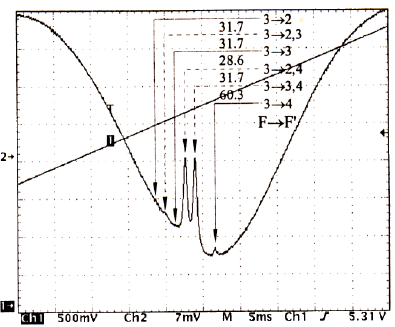
\includegraphics[scale=0.5]{Images/Peaks.png}
	\caption{$_{85}$Rb observed spectrum for $F = 3 \rightarrow F' = 2, \, 3, \, 4$. The transitions to states with two numbers refer to crossover peaks.\cite{manual}}
	\label{fig:Peaks}
\end{figure}
\begin{figure} [!h]
	\centering
	\insertFigure{Images/MOT.png}
	\caption{The MOT setup.\cite{manual}}
	\label{fig:MOT}
\end{figure}
%\section{Procedure} \label{sec:Proc}
\section{Measurements}

\subsection{Laser beam diameter}
Using a movable razor blade and a powermeter, we measured the intensity as a function of the displacement of the blade along an axis perpendicular to the beam propagation direction. The results are collected in Table \ref{table:beampower}. Fitting a function of the form
\begin{alignat*}{2}\label{erf}
f(x) &= \mathrlap{P + A \cdot \text{erfc}(B\cdot x - C),}
\shortintertext{we found}
P &= & 0.0066 \pm 0.0005,\\
A &= & 0.748\pm 0.016,\\
B &= & 4.681 \pm 0.095,\\
C &= & 187.573 \pm 3.829.
\end{alignat*}
\iffalse%Old fitting with constant +- 0.01 as errors
P &= & 0.012 \pm 0.009,\\
A &= & 0.735 \pm 0.007,\\
B &= & 4.942 \pm 0.133,\\
C &= & 198.039 \pm 5.317.
\fi
%TODO Any units for these values? Remember these values are still inside a sentence, so proper punctuation is still necessary.
\begin{table}
\centering
\begin{tabular}{|c|c|}
\hline
Position (cm)	& Power (mW)\\
\hline
$39.4 \pm 0.05$	&	$1.58 \pm 0.08$\\ 	\hline
$39.5 \pm 0.05$	&	$1.57 \pm 0.08$\\ 	\hline
$39.6 \pm 0.05$	&	$1.52 \pm 0.08$\\ 	\hline
$39.7 \pm 0.05$	&	$1.40 \pm 0.07$\\ 	\hline
$39.8 \pm 0.05$	&	$1.07 \pm 0.05$\\ 	\hline
$39.9 \pm 0.05$	&	$0.62 \pm 0.03$\\ 	\hline
$40.0 \pm 0.05$	&	$0.25 \pm 0.01$\\ 	\hline
$40.1 \pm 0.05$	&	$0.10 \pm 0.01$\\ 	\hline
$40.2 \pm 0.05$	&	$0.04 \pm 0.01$\\	\hline
$40.3 \pm 0.05$	&	$0.01 \pm 0.01$\\	\hline
$40.4 \pm 0.05$	&	$0.00 \substack{+0.01 \\ -0.00}$\\	\hline
\end{tabular}
%TODO These uncertainties need to be much larger, we saw a lot more deviations for these during measurement taking. I guess we'll estimate some kind of relative error for all of these to pretend we actually quantified uncertainty then and there.
%Five percent looks good, something comparable error was measured 
\caption{Beam power as a function of position of the razor blade. The errors were estimated to be around 5\% by repeated measurements.}
\label{table:beampower}
\end{table}
This results in a width %http://people.fjfi.cvut.cz/blazejos/public/ul7en.pdf
\begin{equation}
w = 0.3021 \text{ cm } \pm 0.0061 \text{ cm} \nonumber
\end{equation}
\subsection{Size of MOT}
\begin{figure}
\centering
\insertFigure{Images/MOT_w_scale_crop2.png}
\caption{Photo of the MOT merged with photo of the scale.}
\label{fig:mot_w_scale}
\end{figure}
To get an estimate on the MOT size we took a picture of, we used a scale put in the focus to convert distances in pixels to centimeters. By choosing two points $\SI[separate-uncertainty = true]{30.0 \pm 0.5 }{\milli\meter}$ from each other in the image (the error due to the width of the millimeter lines on the scale and the two points not at the same distance from the edge of the ruler), the image viewer software showed $742.2$ pixels. Then
\begin{equation}
1 \text{~px} = \SI[separate-uncertainty = true]{40.42 \pm 0.67}{\micro\meter} \nonumber
\end{equation}
As visible on Figure \ref{fig:mot_w_scale}, the MOT has different horizontal and vertical size values. The directly measured width and height for the MOT are
\begin{align*}
h &= (72 \pm 2)  \, \text{px}\\
w &= (57 \pm 2)  \, \text{px} 
\end{align*}
We chose to approximate the volume by an ellipsoid with one axis half the height ($c$) and two axes half the width ($a$, $b$) each.
\begin{align*}
a, b &= \SI[separate-uncertainty = true]{1.15 \pm 0.04}{\milli\meter} \\
c &=  \SI[separate-uncertainty = true]{1.46 \pm 0.05}{\milli\meter} \\
V &= \frac{4}{3} \pi a b c = \SI[separate-uncertainty = true]{8.09 \pm 0.52 }{\cubic\milli\meter}
\end{align*}
\subsection{Changing the magnetic field}
To measure the MOT fluorescence as a function of the magnetic field, we changed the current flowing through the coils. Figure \ref{fig:magnetic} shows our results. To get a visible MOT, we had to set the current to a minimal value of around $0.9$ A, below this the system fails to trap the moving atoms; from this point, the fluorescence grew proportional to the current to a good approximation, up to $4.6$ A. The background fluorescence has been previously measured and substracted from the data.
\begin{figure}
\centering
\insertFigure{Images/magnetic_dependence_wo_linear.png}
\caption{The dependency of MOT luminosity on the current flow through the coils and thus the strength of the magnetic field.}
\label{fig:magnetic}
\end{figure}
%TODO What is the dependence of the magnetic field with current flow? Should we investigate this or not?
\subsection{Loading behaviour}
\begin{figure}
\centering
\insertFigure{Images/mot_buildup.png}
\caption{Example of data points exported from the oscilloscope, with fitted function (red).}
\label{fig:buildup}
\end{figure}
After replacing the powermeter with a photodiode and showing its signal on an oscilloscope, we used the data from 6 MOT buildup events to find the loading time. As it is known,\cite{inexpensive} the number of trapped atoms changes as
\begin{equation}\label{eq:load}
N(t) = N_0 \big( 1 - e^{-\frac{t}{\tau}} \big),
\end{equation}
where $\tau$ is the loading time, $N_0$ is the maximal number of atoms in the trap. The cross-section is related to $\tau$ if there is only $\ce{Rb}$ in the vacuum chamber (which we assume):
\begin{equation}\label{eq:cross-section}
\frac{1}{\tau} = n_{\text{Rb}} \sigma_{\text{Rb}} v_{\text{Rb}},
\end{equation}
where $n_{\text{Rb}}$ is the number density, $v_{\text{Rb}}$ is the average velocity of the $\ce{Rb}$ vapor (in the following, the subscript Rb is ignored).\\
As the luminescence-time signal also follows Eqn. \ref{eq:load}, by fitting such a function to the oscilloscope data we have gathered yields $\tau$:
\begin{equation}
\tau = (0.268 \pm 0.006) \, \text{s}\nonumber
\end{equation}
With the recorded temperature $T = (293.55 \pm 0.05) \, K$ and pressure $p = (8.09 \pm 0.01)\cdot 10^{-8} \, \text{mbar}$,
%mass of 85 Rb: 84.911 amu = 141.037*10^-27 kg
\begin{equation}
v = \sqrt{\frac{2kT}{m}} = (293.545 \pm 0.025) \, \frac{\text{m}}{\text{s}} \nonumber
\end{equation}
The number density $n$ can be calculated from the ideal gas law:
\begin{equation}
n = \frac{N}{V} = \frac{p}{kT} = (1.99704 \pm 0.00250)\cdot 10^{15} \, \frac{1}{\text{m}^3}\nonumber
\end{equation}
Finally, the cross-section:
\begin{equation}
\sigma = \frac{1}{n \tau v} = (6.355 \pm 0.131) \cdot 10^{-18} \, \text{m}^2
\end{equation}
\section{Conclusion}
%TODO order of appearance!
\begin{thebibliography}{9}
\bibitem{inexpensive}
C. Wieman, G. Flowers and S.Gilbert, Am. J. Phys. \textbf{63} (1995).
\bibitem{manual}
Unspecified Author, \textsl{FP Experiment: Rubidium MOT} (University of Bonn, 2014).
\bibitem{metcalf}
H. Metcalf and P. van der Straten, \textsl{Laser Cooling and Trapping} (Springer, 1999).
\bibitem{Wieman}
C. Wieman and G. Flowers, American Journal of Physics 63 (1995), pp.317-30.
\bibitem{mag}
A. Wolski, \textsl{Maxwell's equations for magnets} (University of Liverpool, 2014), \url{https://arxiv.org/pdf/1103.0713.pdf}.
\bibitem{Foot}
C. J. Foot, \textsl{Atomic Physics} (Oxford University Press, New York, 2005).
\bibitem{demtroder}
W. Demtröder, \textsl{Laser Spectroscopy, Basic Concepts and Instrumentation} (Springer, 2003).%Third Edition
\bibitem{laserdiode}
\textsl{Physics Fundamentals: Laser Diode Characteristics}, \url{https://www.sukhamburg.com/download/fundamentals-laserdiodes.pdf}
\iffalse
%Leaving this here as examples for referencing different media
\bibitem{book}
K. Siegbahn, \textsl{Alpha-, beta-, and gamma-ray spectroscopy, Vol. 2} (North Holland Publishing Company, Amsterdam, 1965).
\bibitem{booklet}
Unspecified author, \textsl{Advanced Laboratory Course (physics601): Description of Experiments} (University of Bonn, 2018).
 \bibitem{link}
 W. U. Boeglin, \textit{Scintillation Detectors}, WWW Document, \url{http://wanda.fiu.edu/teaching/courses/Modern_lab_manual/scintillator.html}.
\bibitem{pdf_on_website}
Unspecified author, \textsl{Gamma Ray Spectroscopy} (University of Florida, 2013), \url{https://www.phys.ufl.edu/courses/phy4803L/group_I/gamma_spec/gamspec.pdf}.
\bibitem{journal}
E. Ermis and C. Celiktas, International Journal Of Instrumentation Science 1, (2013), pp.54-62.
%alternative url: https://en.wikipedia.org/wiki/Constant_fraction_discriminator
\bibitem{}
M. Nakhostin, \textsl{Signal Processing for Radiation Detectors} (John Wiley $\&$ Sons, 2018), p. 298\footnote{Relevant pages (chapter 6) available for preview under\\ \url{https://books.google.de/books?id=Lrg4DwAAQBAJ}}.
%Mohammad Nakhostin
\bibitem{}
W. R. Leo, \textsl{Techniques for Nuclear and Particle Physics Experiments} (Springer-Verlag, 1987), p. 305.
%William R. Leo
\bibitem{}
A. C. Melissinos, J. Napolitano, \textsl{Experiments in Modern Physics, 2\textsuperscript{nd} edition} (Academic Press, San Diego, 2003), pp 419-21.
\fi
\end{thebibliography}
\end{document}